\documentclass[ruledheader,noindentfirst,anapcustomindent,abntfigtabnum,tocpage=plain]{def_and_cls/abnt}
\usepackage{amsmath, amssymb, amsthm, verbatim, amsfonts, amstext}
%\usepackage[latin1]{inputenc}
\usepackage[brazilian]{babel}
\usepackage[utf8]{inputenc}
\usepackage[T1]{fontenc}
\usepackage{styles/dropping}
\usepackage{graphicx}
\usepackage[hang,small,bf]{caption}
\usepackage[abnt-etal-list=0,abnt-etal-text=it,abnt-and-type=&,abnt-emphasize=bf,abnt-full-initials=yes,alf,bibjustif]{styles/abntcite}
\usepackage{fancyhdr}
\usepackage{makeidx}
\usepackage[none]{hyphenat}
\usepackage{color}
\usepackage{subfig}
\usepackage{styles/algorithms}
\usepackage{algorithmic}
\usepackage{mdwlist}
\usepackage{bm}
\usepackage[titletoc,title]{appendix}
\usepackage{ltxtable}
\usepackage{longtable}
\usepackage{supertabular}
\usepackage{indentfirst}
\usepackage{color}
\usepackage{icomma}
\usepackage{siunitx}
\usepackage{biblatex}
\addbibresource{../bib/mybibliography.bib}

\sloppy


%
%Tradução do pacote Algorithm para portugues
%
\renewcommand{\algorithmicrequire}{\textbf{Entrada:}}
\renewcommand{\algorithmicensure}{\textbf{Saída:}}
\renewcommand{\algorithmicend}{\textbf{fim}}
\renewcommand{\algorithmicif}{\textbf{se}}
\renewcommand{\algorithmicthen}{\textbf{então}}
\renewcommand{\algorithmicelse}{\textbf{senão}}
\renewcommand{\algorithmicelsif}{\algorithmicelse \, \algorithmicif}
\renewcommand{\algorithmicendif}{\algorithmicend \, \algorithmicif}
\renewcommand{\algorithmicfor}{\textbf{para}}
\renewcommand{\algorithmicforall}{\textbf{para todo}}
\renewcommand{\algorithmicdo}{\textbf{fazer}}
\renewcommand{\algorithmicendfor}{\algorithmicend \, \algorithmicfor}
\renewcommand{\algorithmicwhile}{\textbf{enquanto}}
\renewcommand{\algorithmicendwhile}{\algorithmicend \, \algorithmicwhile}
\renewcommand{\algorithmicloop}{\textbf{laço}}
\renewcommand{\algorithmicendloop}{\algorithmicend \, \algorithmicloop}
\renewcommand{\algorithmicrepeat}{\textbf{repetir}}
\renewcommand{\algorithmicuntil}{\textbf{até}}
\renewcommand{\algorithmiccomment}[1]{\{#1\}}
\renewcommand{\listalgorithmname}{Lista de Algoritmos}
\floatname{algorithm}{Algoritmo}
%%%%%%%%%%%%%%%%%%%%%%%%%%%%%%%%%%%%%%%%%%%%%%%%%%%%%%%%%%%%%%%%%%%%%%%%%%%%%%%%%%%

\makeindex

%%%% O arquivo modelosCAP.tex possui as definições para ciação do estilo de capítulo (fonte de título, barras horizontais, etc.)
% ele não gera texto de saída, é um arquivo de configuração somente
%
%Estilo de formatação de capítulos

\makeatletter
\newcommand{\thechapterwords}
{ \ifcase \thechapter\or 1\or 2\or 3\or 4\or 5\or6\or 7\or 8\or 9\or 10\or 11\fi}

\def\@makechapterhead#1{%
\vspace*{10\p@}%
{\parindent \z@  \reset@font

\scshape \@chapapp{} \thechapterwords
\quad %
\par\nobreak
\vspace*{10\p@}%
\interlinepenalty\@M
\hrule
\vspace*{10\p@}%
\Huge \bfseries #1\par\nobreak
\par
\vspace*{10\p@}%
\hrule
\vskip 40\p@
}}
\def\@makeschapterhead#1{%
\vspace*{10\p@}%
{\parindent \z@ \centering \reset@font
\par\nobreak
\vspace*{10\p@}%
\interlinepenalty\@M
\hrule
\vspace*{10\p@}%
\Huge \bfseries #1\par\nobreak
\par
\vspace*{10\p@}%
\hrule
\vskip 40\p@
%\vskip 100\p@
}}
%%%%%%%%%%%%%%%%%%%%%%%%%%%%%%%%%%%%%%%%%%%%%%%FIM DO PREAMBULO%%%%%%%%%%%%%%%%%%%%%%%%%%%%%%%%%%%%%%%%%%%%%%%%%%%%%%%%%%%%%%%%%%


\begin{document}

%%%%% IMPORTANTE: ALTERA O TEXTO ENTRE ARIAL E TIMES NEW ROMAN (ALTERNAR OS COMENTÁRIOS)
%
%%%%%%%%%%%%%%%%%%%%%PARA UTILIZAR ARIAL%%%%%%%%%%%%%%%%%%%%%%%
%
\fontfamily{phv}                    %fonte Arial
\renewcommand{\rmdefault}{phv}      %
%
%%%%%%%%%%%%%%%%%%%%%PARA UTILIZAR TIMES%%%%%%%%%%%%%%%%%%%%%%%
%
%\fontfamily{ptm}               %fonte Times
%\renewcommand{\rmdefault}{ptm} %
%
%%%%%%%%%%%%%%%%%%%%%%%%%%%%%%%%%%%%%%%%%%%%%%%%%%%%%%%%%%%%%%%

%%%%%%%%%%%%%Arquivos .tex com os elementos pré-textuais
%
\thispagestyle{empty}

\vfill
 \begin{center}
    \begin{figure}[t]
     \centering
            
\includegraphics[width=5cm]{figures/IF_logo.eps}\\[-0.1in]
     \end{figure}

    {\large\bfseries INSTITUTO FEDERAL DE EDUCAÇÃO, CIÊNCIA E TECNOLOGIA DO CEARA} \\
    {\large\bfseries PRÓ-REITORIA DE ENSINO} \\
    {\large\bfseries COORDENADORIA DE TELEMÁTICA DO CAMPUS MARACANAÚ}  \\ 
    {\large\bfseries BACHARELADO EM CIÊNCIA DA COMPUTAÇÃO}  \\ 

    \vspace*{1in}
    \begin{large} \bfseries FELIPE MARCEL DE QUEIROZ SANTOS \end{large}\\[0.4in]

    \vspace*{4cm}
    \noindent \\
    \large\bfseries{TÍTULO DO TRABALHO} \\
    \vfill
    \large\bfseries{ MARACANAÚ \\ 2015}
\end{center}

\normalsize
\begin{titlepage}
\vfill
\begin{center}

    {\large FELIPE MARCEL DE QUEIROZ SANTOS\\}
    \vspace{2cm}
    {\Large \textsc{TiTULO DO TRABALHO}\\}
    \vspace{1cm}
    \hspace{.45\linewidth}
    \begin{minipage}{.50\linewidth}

            Monografia submetida à Coordenadoria de Telemática e à Coordenadoria do Curso de Bacharelado 
            em Ciência da Computação do Instituto Federal do Ceará - Campus Maracanaú, como requisito 
            parcial para obtenção do grau de Bacharel em Ciência da Computação.

            \vspace{0.5 cm}

            Área de pesquisa: Aprendizagem de Máquina

            \vspace{0.5 cm}

            Orientador:D.r AMAURI HOLANDA SOUZA JUNIOR
    
    \end{minipage}

    \vspace{2cm}
    \vfill
    {\large Maracanaú\\ 2015}
\end{center}

\end{titlepage}
\begin{folhadeaprovacao}
\setlength{\ABNTsignthickness}{0.2pt}
\setlength{\ABNTsignskip}{1.7cm}

\begin{center}

\includegraphics[width=2.5cm]{figures/brasao_republica.eps}\\
%
\includegraphics[width=5cm]{figures/IF_logo.eps}\\ %outros brasões
%
\includegraphics[width=5cm]{figures/IF_logo2.eps}\\%outros brasões

            {INSTITUTO FEDERAL DE EDUCAÇÃO, CIÊNCIA E TECNOLOGIA DO CEARÁ} \\
            {COORDENAÇÃO DE PÓS-GRADUAÇÃO EM ENGENHARIA DE TELECOMUNICAÇÕES}  \\

    \vspace{1.5cm}
                                    {FELIPE MARCEL DE QUEIROZ SANTOS}\\
    \bfseries{}
\end{center}

Esta Monografia foi julgada adequada para a obten\c{c}\~{a}o do Grau de Bacharel em Ciência da Computação, sendo aprovada pela Coordenadoria de Telemática e pela Coordenadoria do curso de Bacharelado em Ciência da Computação do Campus Maracanaú do Instituto Federal de Educação, Ciência e Tecnologia do Ceará e pela banca examinadora:

    \vspace{0.15cm}
    \assinatura{Orientador: Prof. Dr. Amauri \\ Instituto Federal do Ceará - IFCE}
    \assinatura{Prof. Dr. Huguinho \\ Instituto Federal do Ceará - IFCE}
    \assinatura{Prof. Dr. Zezinho \\ Instituto Federal do Ceará - IFCE}
    \assinatura{Prof. Dr. Luizinho \\ Instituto Federal do Ceará - IFCE}
    \vspace{0.15cm}%\vfill

    \begin{center}
        Fortaleza, 06 de Abril de 2013
    \end{center}
\end{folhadeaprovacao}
\vspace*{15cm}

\hfill Dedico este trabalho ...\\
\chapter*{Agradecimentos}
%\thispagestyle{empty}


\begin{flushright}
\begin{minipage}[r]{10cm}
\vspace{18cm}
``A mente que se abre a uma nova idéia jamais voltará ao seu tamanho original''.
\begin{flushright}
Albert Einstein
\end{flushright}
\end{minipage}
\end{flushright}
\pagestyle{plain}%%%%% Utilizar ESTILO PLAIN AQUI%%%%%%%
\chapter*{Resumo}

\noindent Este trabalho visa desenvolver a especificação de um sistema 'gimbal' open-source e open-hardware de baixo custo visando tornar esta tecnologia mais acessível. A demanda foi identificada pelo integrante Breno, ao perceber que os fabricantes cobravam preços muito altos inclusive por equipamentos amadores. \\
Especificamos o uso do microcontrolador ATMega328P por ser fácil de obter e estar presente na plataforma Arduino, ao qual a maioria dos usuários tem acesso. O OS escolhido é o armOS, por ter capacidades de tempo real, e que se comunicará com os periféricos: um giroscópio, acelerômetro, botões, servo-motores e LEDs.
\chapter*{Abstract}


\noindent This work presents...

%%%Comandos para criação automática das listas
%
\tableofcontents
\listoffigures
\listoftables

%%%Comandos para criar outras listas não suportadas pelo pacote ABNTex%%%
%
%%%%%%%%%%%%%%%%%%%%%%%%%%%%%%%%%%%%%%%%%%%%%%%%%%%%%%%%%%%%%%%%%%%%

%Capítulos passam a ter páginas numeradas
%
\pagestyle{fancy}

%resseta os contadores de capítulo e seção
%
\renewcommand{\chaptermark}[1]{\markboth{#1}{}}
\renewcommand{\sectionmark}[1]{\markright{\thesection\ #1}}

%%%%%%%%%%%%%%NÃO LEMBRO O QUE FAZ, APARENTEMENTE NADA, TESTAR DEPOIS
%\fancyhf{}%
%\fancyhead[RO,LE]{\large\slshape\thepage}%
%\fancyhead[CE]{\large\slshape\leftmark}%
%\fancyhead[CO]{\large\slshape\rightmark}%


%%% Outros arquivos .tex. É acoselhável utilizar vários arquivos, pelo menos um por capítulo
\chapter{Introdução}\label{CAP:introducao}
%\thispagestyle{empty}

Este documento consiste de um modelo basico para a producao de documentos academicos, seguindo as normas ABNT. 

Nao e abordado o estudo do LaTex neste template. Sugerimos a leitura do texto em \citeonline{Oetiker:1995}. O uso do LaTex e aconselhavel devido a sua qualidade grafica, facil referenciacao, criacao de listas, indices, referencias bibliograficas e escrita matematica profissional. Porem, nao e obrigatorio o uso deste template, apenas as orientacoes de formatação segundo as normas ABNT devem ser obrigatoriamente seguidas.

Uma observação em particular é a de que, no pacote ABNTex, as referências diretas devem utilizar o comando ``citeonline''. Referências indiretas utilizam o comando ``cite''.

Exemplo de citacao direta: Uma otima fonte de estudo para compreender o LaTex e apresentada por \citeonline{Oetiker:1995}. 

Exemplo de citação indireta: Existem boas fontes de pesquisa para entendimento do LaTex \cite{Oetiker:1995}, estas incluem documentação online disponível na web.

\section{Motivação e objetivos}


 
\section{Contribuicoes}




\section{Producao cientifica}


\section{Organizacao da tese}

\noindent \textbf{Capitulo \ref{CAP2}}: descricao...

\noindent \textbf{Capitulo \ref{CAP3}}: descricaoo...

\noindent \textbf{Capitulo \ref{CAP4}}: descricao...

\noindent \textbf{Capitulo \ref{CAP5}}: descricao...
\chapter{Métodos de Kernel}
\label{CAP2}


Este capítulo tem como objetivo 


\section{Kernel em análise de padrões}\label{Sub:equa}

Em análise de padrões, temos como objetivo detectar automaticamente padrões em um conjunto de dados de um determinado problema. Por padrões, podemos entender qualquer relação ou regularidades inerentes à alguma estrutura em uma fonte de dados. Essa análise geralmente é feita a partir dos valores de entrada e suas respectivas saídas(no caso da aprendizagem supervisionada) fornecidas no problema. Essas informações podem formar padrões em que se torna possível verificar o valor de uma saída dada uma nova entrada fornecida pelo usuário. 

Diversos problemas podem ser resolvidos utilizando esta abordagem, categorização de textos, análise de sequências de DNA, reconhecimento de escrita, por exemplo.

A abordagem de análise de padrões utilizando métodos de kernel se baseia em adaptar os dados de entrada em um espaço característico adequado e nos algoritmos usados para descobrir os padrões do problema. Levando em conta isso, podemos pensar que qualquer solução com métodos de kernel é composta por estas duas partes: uma em que é feito o mapeamento nesse espaço característico e a outra em que é executado o algoritmo de aprendizagem para detectar os padrões neste espaço. A ideia por trás desta abordagem é poder mapear os dados em um espaço em que possamos 

Uma das principais caracerísticas desses métodos é o atalho computacional que pode ser utilizado, tal atalho é conhecido como função de kernel.


O Kernel  é uma função de mapeamento de dados em dimensões superiores com a motivação de torná-los mais fáceis de separar ou estruturá-los de maneira mais adequada. Essas funções podem ser utilizadas nas tarefas de reconhecimento de padrões. 

\begin{equation}\label{Eq:multiplicacao}
%
Z = X \cdot Y,
%
\end{equation}
%
em que $Z$, $X$ e $Y$ são variáveis complexas. A referenciação à Equação (\ref{Eq:multiplicacao}) é feita por meio do comando ``ref''. O mesmo vale para outros tipos de elementos.

\subsection{Exemplo de uma equação mais complexa}

  Equações mais complexas podem ser mais facilmente escritas com uso do programa TexAide. Como, por exemplo,

    \begin{equation}\label{Eq:sqrt_gamma_X}
    f_{\Gamma ^{{1 \mathord{\left/
    {\vphantom {1 2}} \right.
    \kern-\nulldelimiterspace} 2}} } (x;\alpha ,\lambda ) = \frac{{2\lambda ^\alpha  }}{{\Gamma (\alpha )}}x^{2\alpha  - 1} \exp \left( { - \lambda x^2 } \right).
    \end{equation}
    \[
    \alpha ,\lambda > 0.
    \]
    %
    em que $\Gamma(\cdot)$ é a função Gama. O programa TexAide é semelhante ao \textit{MathType} do Office, porém ao copiar e colar a equação em um arquivo tex, é gerado o código em LaTex referente a esta equação.

\section{Tabelas}

Tabelas são essenciais na apresentação de dados. A Tabela \ref{Tb:X_models} mostra um exemplo do uso deste tipo de elemento. Vale ressaltar que não é aconselhável o uso de linhas verticais em trabalhos acadêmicos e de pesquisa.

\begin{table}[h]
 \caption{Modelos estatísticos e suas relações.}%
 \label{Tb:X_models}
  \centering
\begin{tabular}{c c c c c}
 \hline
 &&&&\\
                                             &$\alpha ,\lambda  > 0$    &                               &$\alpha ,\lambda \rightarrow\infty$  &Homogêneo \\
                                             &$\gamma  \to 0$           & Heterogêneo                   &$\alpha / \lambda \rightarrow \beta$ & \\
                                             &$\mathop  \to \limits^D $ & $\sqrt\Gamma(\alpha,\lambda)$ &$\mathop  \to \limits^P $            &$\sqrt\beta$        \\
$\mathcal{N}^{-1/2}(x;\alpha,\gamma,\lambda)$& & & &\\
                                             &$\mathop  \to \limits^D $ & $\Gamma^{-1/2}(\alpha,\gamma)$&$\mathop  \to \limits^P $   &$\sqrt{\zeta^{-1}}$ \\
                                             &$\lambda \to 0$           &  Extremamente                 &$-\alpha / \gamma \rightarrow \zeta^{-1}$ & \\
                                             &$-\alpha ,\gamma   > 0$   &  Heterogêneo                  &$-\alpha ,\gamma \rightarrow\infty$ &Homogêneo \\
 &&&& \\
 \hline
 &&&&\\
                                             &$\alpha ,\lambda  > 0$    &                               &$\alpha ,\lambda \rightarrow\infty$  &Homogêneo \\
                                             &$\gamma  \to 0$           & Heterogêneo                   &$\alpha / \lambda \rightarrow \beta$ & \\
                                             &$\mathop  \to \limits^D $ &$\mathcal{K}_A(\alpha,\lambda,n)$&$\mathop  \to \limits^P $&$\sqrt\Gamma(n,n/\beta)$        \\
$\mathcal{G}_A(z;\alpha,\gamma,\lambda,n)$   & & & &\\
                                             &$\mathop  \to \limits^D $ & $\mathcal{G}_A^0(\alpha,\gamma,n)$&$\mathop  \to \limits^P $&$\sqrt\Gamma(n,n\zeta)$  \\
                                             &$\lambda \to 0$           &  Extremamente                 &$-\alpha / \gamma \rightarrow \zeta$ & \\
                                             &$-\alpha ,\gamma   > 0$   &  Heterogêneo                  &$-\alpha ,\gamma \rightarrow\infty$ &Homogêneo \\
&&&&   \\
 \hline

\end{tabular}
\end{table}


A Figura \ref{Fig:1} mostra o exemplo do uso do comando ``subfigure''. Apesar de aceitar diferentes tipos de imagens. É preferível que as imagens estejam no formato .eps. Isso garante que a imagem impressa seja exatamente aquela visualizada, como acontece com arquivos pdf.

\begin{figure}[!ht]
\centering
\subfloat[]{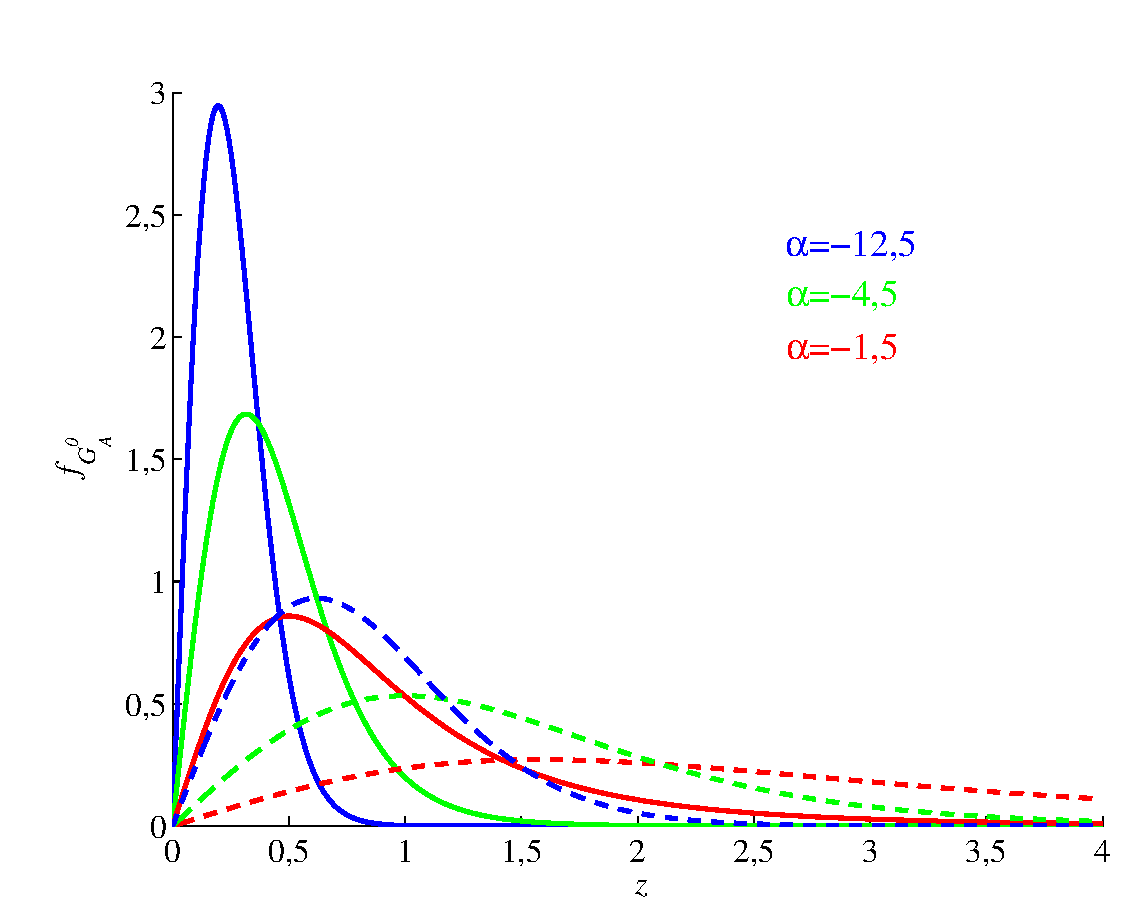
\includegraphics[scale=.65]{figures/fig1.eps}}\\
\subfloat[]{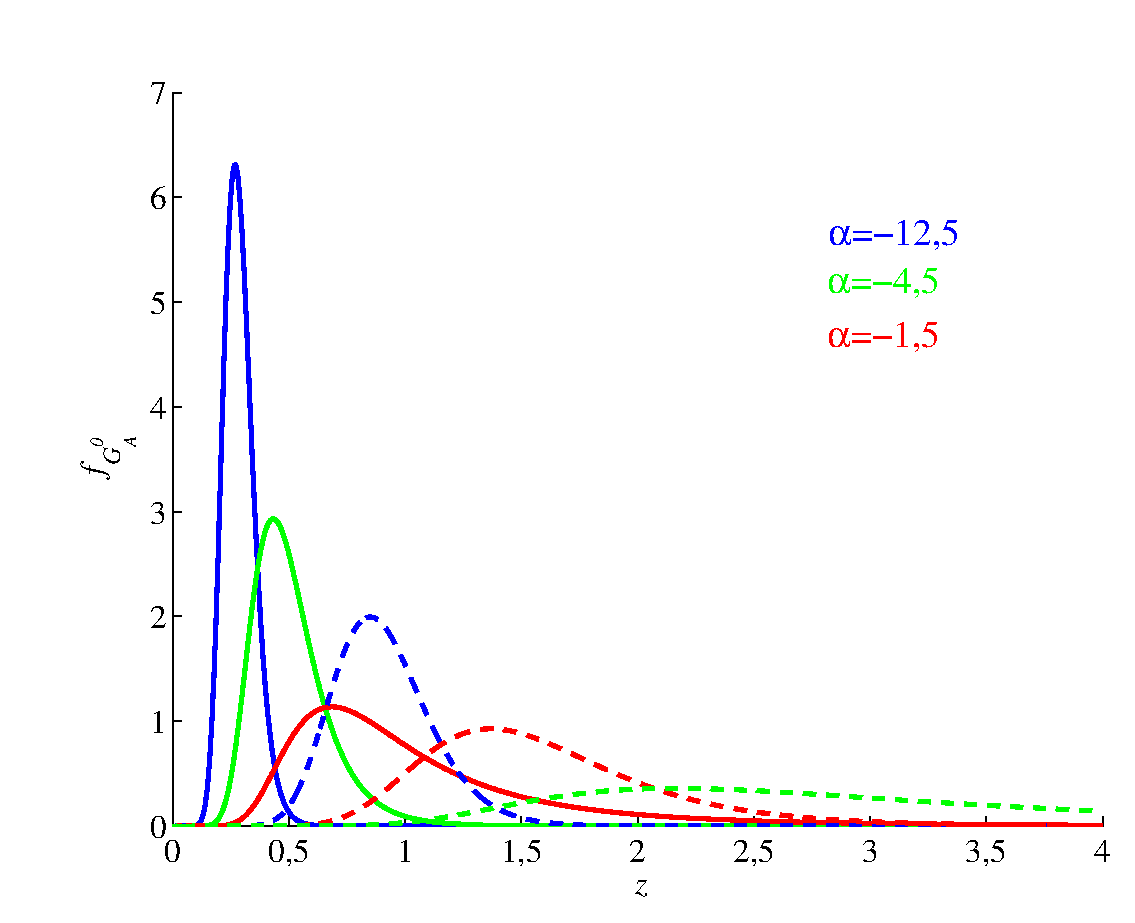
\includegraphics[scale=.65]{figures/fig2.eps}}
\caption{ Curvas de funções de probabilidade: (a) exemplo 1, (b) exemplo 2.} \label{Fig:1}
\end{figure}
    \chapter{Metodologia do trabalho}
\label{CAP3}


Esta seção trata das fases do trabalho: como deverão ser executadas e em que sequência.


\section{Montar a estrutura}\label


Linha Zhiyun Smooth só serve para celulares, o nosso estabilizador servirá para câmeras semi-profissionais  também
Por serem feitos para câmeras profissionais, precisam de mais robustez, por isso, custam mais caro:
Linha Gimbal DJI RS
Valor acima de 2500 reais
Linha S Leeremi
Valor acima de 1000 reais


\section{Montar a estrutura 2}\label


\chapter{Especificação de requisitos}

\label{CAP4}

\section{Requisitos funcionais}

Neste capítulo serão descritas as necessidades básicas levantadas para que o projeto funcione como esperado.

Os requisitos inicialmente propostos foram os seguintes


\begin{table}[H]
\caption{}
\label{tab:requisitos}
\begin{tabular}{|c|c|}
\hline
{ \textbf{Propósito}}       & { Estabilizar uma câmera em 3 eixos}                                                                       \\ \hline
{ \textbf{Entradas}}        & { \begin{tabular}[c]{@{}c@{}}Botão de energia, botão de trava,\\ acelerômetro e giroscópio\end{tabular}} \\ \hline
{ \textbf{Saídas}}          & { 3 motores de passo}                                                                                      \\ \hline
{ \textbf{Funções}}         & { Estabilizar uma câmera em tempo real}                                                                    \\ \hline
{ \textbf{Performance}}     & { Ajusta a posição a cada 10ms}                                                                            \\ \hline
{ \textbf{Custo}}           & { R\$250,00}                                                                                               \\ \hline
{ \textbf{Potência}}        & { 1W}                                                                                                      \\ \hline
{ \textbf{Tamanho e massa}} & { Até 200g, aproximadamente 30cm x 5cm x 5cm}                                                              \\ \hline
\end{tabular}
\end{table}

Ao longo do desenvolvimento diversos requisitos foram alterados para melhor enquadrarem os objetivos de longo prazo do projeto: 
\begin{table}[H]
\caption{}
\label{tab:requisitos}
\begin{tabular}{|c|c|}
\hline
{ \textbf{Propósito}}       & { Estabilizar uma câmera em 3 eixos}                                                                       \\ \hline
{ \textbf{Entradas}}        & { \begin{tabular}[c]{@{}c@{}}Botão de energia, botão de trava,\\ acelerômetro e giroscópio\end{tabular}} \\ \hline
{ \textbf{Saídas}}          & { 3 motores de passo, 4 leds}                                                                                      \\ \hline
{ \textbf{Funções}}         & { Estabilizar uma câmera na taxe de quadros da camera}                                                                    \\ \hline
{ \textbf{Performance}}     & { Ajusta a posição a cada 16,6ms}                                                                            \\ \hline
{ \textbf{Custo}}           & { R\$350,00}                                                                                               \\ \hline
{ \textbf{Corrente}}        & { ~16W}                                                                                                     \\ \hline
{ \textbf{Tamanho e massa}} & { Até 500g, aproximadamente 30cm x 5cm x 5cm}                                                              \\ \hline
\end{tabular}
\end{table}


\section{Requisitos não-funcionais}



\chapter{Desenvolvimento do trabalho}

Este capítulo tem como objetivo explicitar quais foram as decisões de projeto que foram tomadas ao longo do desenvolvimento do sistema.

\section{Tecnologias utilizadas}


\subsection{ATmega328P}
Motivação:
Fácil de implementar, ajuda na ideia de open-hardware
Memória programável já dentro do sistema (alguns ATs não têm)
Não é caro (maior parte do custo será nos componentes mecânicos)
Consumo de energia baixo (22mW) em relação à potência proposta (de 1W)

\subsection{Sistema Operacional}
Como o projeto requer controle em tempo real da câmera, é necessário usar um RTOS (real time operating system).
Entre os SOs apresentados, o mais adequado para o controlador Gimbal é o ARM OS.

\subsection{Interface}
SPI (GPIO das placas feitas pela Arduino):
Giroscópio: dados posicionais
Acelerômetro: dados posicionais
Botões (ao menos dois): interface com o usuário
LED (depuração): interface com o usuário
USB:
Carregamento: fazer o código rodar no Arduino 
Depuração: do código na placa

\subsection{Ambiente de desenvolvimento e depuração}
Usaremos as bibliotecas de cada sensor e motor a ser usado, para facilitar a integração
Não há necessidade de sistema de arquivos, já que os dados são tratados ativamente
Usaremos os drivers de interface com o GPIO fornecidos pelo SO
A depuração será feita em cada camada de maneiras diferentes: 
Simulação → aplicação 
QEMU → SO 
LEDs → hardware 

\section{Projeto e implementação}

\section{Testes e avaliação}




\chapter{Considerações finais}
\label{CAP6}


Este capítulo descreve as observações posteriores à conclusão do projeto.Este capítulo tem como objetivo 


\section{Conclusão}

\section{Contribuições}

\section{Perspectivas de continuidade}


% \chapter{Referências}

% %\urlstyle{same} % mantém fonte das letras que compõem url

% [1] \textbf{US20130052614A1 - Driver Performance Metric}. Google Patents, 2012. Disponível em <\url{patents.google.com/patent/US20130052614}>. Acesso em 30 de jan. de 2022.

% [2] CAMPO GRANDE, Paulo. \textbf{Novas Tecnologias: Carros Atuais Têm Até 100 Sensores a Bordo}. Revista Quatro Rodas, Brasil, 12 de jun. de 2018. Disponível em <\url{quatrorodas.abril.com.br/noticias/novas-tecnologias-carros-atuais-tem-ate-100-sensores-a-bordo/}>. Acesso em 20 de fev. de 2022.

% % 17 de mar de 
% [3] WIKIMEDIA Foundation. \textbf{OBD-II PIDs}. Wikipedia, 2022. Disponível em <\url{en.wikipedia.org/wiki/OBD-II_PIDs}>. Acesso em 20 de mar. de 2022

% % 9 de set. de 
% [4] FINCO, Nina. \textbf{OBD}: o Que é e Para Que Serve o Protocolo OBD2?. Cobli Blog, 2021. Disponível em <\url{www.cobli.co/blog/o-que-e-protocolo-obd2/}>. Acesso em 20 de mar. de 2022.

% % 25 de nov. de
% [5] BARRETO, Victor. \textbf{What Is OBDII?} History of on-Board Diagnostics. Geotab, 2020 Disponível em <\url{www.geotab.com/blog/obd-ii/}>. Acesso em 20 de mar. de 2022.

% [6] SBT News. \textbf{No Brasil, cerca de 32 pessoas morrem por dia em acidentes de trânsito}. SBT, Brasil, 22 de jan. de 2022. Disponível em <\url{www.sbtnews.com.br/noticia/brasil/194388-no-brasil--cerca-de-32-pessoas-morrem-por-dia-em-acidentes-de-transito#:~:text=Em 2021, foram 11.647 mortes,incidentes por hora no Brasil.}>. Acesso em 23 de abr. de 2022.

% [7] \textbf{ACIDENTES De Trânsito São a Maior Causa De Morte De Pessoas De 5 a 29 Anos}. ONU News. Nações Unidas, 21 de nov. de 2021. Disponível em <\url{news.un.org/pt/story/2021/11/1771092}>. Acesso em 18 de abr. de 2022.

% [8] \textbf{TOTAL Confirmed COVID-19 Deaths}. Our World in Data, 2022. Disponível em <\url{ourworldindata.org/grapher/covid-deaths-income}>
% . Acesso em 18 de abr. de 2022.

% [9] \textbf{Em Quanto Tempo Os Carros Autônomos Serão o Novo 'Padrão'?}. Jaguar Brasil. Disponível em <\url{www.jaguarbrasil.com.br/news/em-quanto-tempo-os-carros-autonomos-serao-o-novo-padrao.html#:~:text=A indústria de pesquisa IHS,pode demorar um pouco mais}>. Acesso em 23 de abr. de 2022.


% [10] \textbf{PREÇO sob demanda do Amazon EC2}. Amazon. Disponível em <\url{aws.amazon.com/pt/ec2/pricing/on-demand/}>. Acesso em 23 de abr. de 2022.


% [11] \textbf{CALCULADORA de preço}. Microsoft Azure. Disponível em <\url{azure.microsoft.com/de-de/pricing/calculator/}>. Acesso em 23 de abr. de 2022.

% [12] PIRES. \textbf{Android OBD-II Reader Application That Uses Pure OBD-II PID's Java API}. GitHub. Disponível em <\url{github.com/pires/android-obd-reader}>. Acesso em 23 de abr. de 2022.

% [13] PAGE, Vanessa. \textbf{Waze: The Pros and Cons}. Investopedia, 12 de jan de 2022. Disponível em <\url{www.investopedia.com/articles/investing/060415/pros-cons-waze.asp#:~:text=Waze uses data from app,that could slow down drivers}>. Acesso em 23 de abr. de 2022.


% [14] \textbf{Scanner Automotivo Conector Obd2 Elm327 Bluetooth}. Mercado Livre, <\url{produto.mercadolivre.com.br/MLB-2147325216-scanner-automotivo-conector-obd2-elm327-bluetooth-_JM#position=1&search_layout=grid&type=pad&tracking_id=509523dc-c530-481c-954c-0ecbe9c6a94c&is_advertising=true&ad_domain=VQCATCORE_LST&ad_position=1&ad_click_id=ODlhMjFlMzctNjQ5Ni00MTg1LWIzYWYtZjk3Y2U5MjlmNjNm}>. Acesso em 23 de abr. de 2022.

% [15] SAIPRASERT, Chalermpol. et al. \textbf{Driver Behaviour Profiling Using Smartphone Sensory Data in a V2I Environment}. 2014 International Conference on Connected Vehicles and Expo (ICCVE), 2014. Disponível em <\url{https://ieeexplore.ieee.org/abstract/document/7297609}>. Acesso em 24 de abr. de 2022.



\chapter{Integração}\label{CAP:integracao}

\label{CAP8}

Como juntar todas as subpartes do projeto é uma outra tarefaimportante de engenharia.

A seguir é descrito como isso pode ser feito.

\section{Compra da placa ATMEGA}
\section{Compra da placa ATMEGA}
\section{Compra da placa ATMEGA}
\section{Compra da placa ATMEGA}
\section{Compra da placa ATMEGA}
\chapter{Conclusão}]

\label{CAP9}


Este capítulo tem como objetivo 


\section{eeeeeeeeeeeeeeeeee}\label{Sub:equa}


%%%% Estilo de citação ABNT e arquivo de bibitens (mybibliography.bib)
% \bibliographystyle{abnt-alf}
% \bibliography{mybibliography}
\printbibliography
\apendice
\include{appendices}


\end{document}